% Author: Izaak Neutelings (Februari, 2020)
% http://texample.net/tikz/examples/tag/circuitikz/
% http://texample.net/tikz/examples/circuitikz/
% https://www.overleaf.com/learn/latex/CircuiTikz_package
% http://texdoc.net/texmf-dist/doc/latex/circuitikz/circuitikzmanual.pdf
% https://repositorios.cpai.unb.br/ctan/graphics/pgf/contrib/circuitikz/circuitikzmanual.pdf
\documentclass[border=3pt,tikz]{standalone}
\usepackage{amsmath} % for \dfrac
\usepackage{physics}
\usepackage{tikz,pgfplots}
\usepackage[siunitx]{circuitikz} %[symbols]
\usepackage[outline]{contour} % glow around text
\usetikzlibrary{arrows,arrows.meta}
\usetikzlibrary{decorations.markings}
\tikzset{>=latex} % for LaTeX arrow head
\usepackage{xcolor}
\colorlet{Icol}{blue!50!black}
\colorlet{Ccol}{orange!90!black}
\colorlet{Rcol}{green!50!black}
\colorlet{Lcol}{violet!90}
\colorlet{loopcol}{red!90!black!25}
\colorlet{pluscol}{red!60!black}
\colorlet{minuscol}{blue!60!black}
\newcommand\EMF{\mathcal{E}} %\varepsilon}
\contourlength{1.5pt}
%\tikzstyle{EMF}=[battery1,l=$\AC_0$,invert]
\tikzstyle{AC}=[sV,/tikz/circuitikz/bipoles/length=25pt,l=$\EMF(t)$]
\tikzstyle{internal R}=[R,color=Rcol,Rcol,l=$r$,/tikz/circuitikz/bipoles/length=30pt]
\tikzstyle{loop}=[->,red!90!black!25]
\tikzstyle{loop label}=[loopcol,fill=white,scale=0.8,inner sep=1]
\tikzstyle{thick R}=[R,color=Rcol,thick,Rcol,l=$R$]
\tikzstyle{thick C}=[C,thick,color=Ccol,Ccol,l=$C$]
\tikzstyle{thick L}=[L,thick,color=Lcol,Lcol,l=$L$,/tikz/circuitikz/bipoles/length=56pt] %inductor
\tikzstyle{thick Z}=[generic,color=Icol,thick,Icol,l=$Z$,fill=Icol!6]



\begin{document}


% AC, R
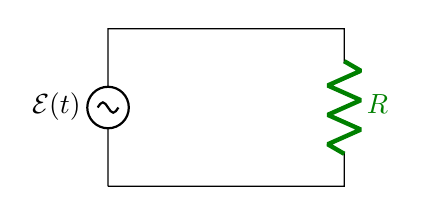
\begin{tikzpicture}
  \def\ang{155}
  \def\a{0.9}
  \def\b{0.8}
  \draw (0,0) to[AC] (0,2) --++(3,0)
              to[thick R] ++(0,-2) -- (0,0);
\end{tikzpicture}


% AC, C
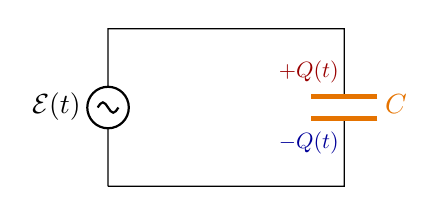
\begin{tikzpicture}
  \def\ang{155}
  \def\a{0.9}
  \def\b{0.8}
  \draw (0,0) to[AC] (0,2) --++(3,0)
              to[thick C] ++(0,-2) -- (0,0);
  \node[minuscol,scale=0.8] at (2.55,0.55) {$-Q(t)$};
  \node[pluscol,scale=0.8] at (2.55,1.45) {$+Q(t)$};
\end{tikzpicture}


% AC, L
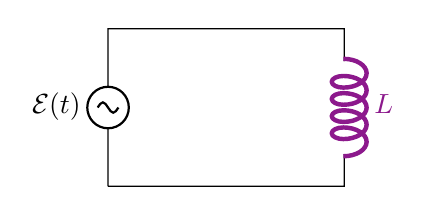
\begin{tikzpicture}
  \def\ang{155}
  \def\a{0.9}
  \def\b{0.8}
  \draw (0,0) to[AC] (0,2) --++(3,0)
              to[thick L] ++(0,-2) -- (0,0);
\end{tikzpicture}


% AC, RCL series
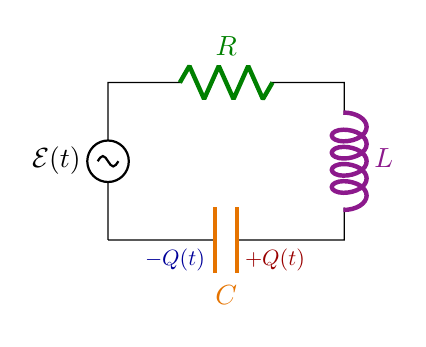
\begin{tikzpicture}
  \def\ang{120}
  \def\a{1.0}
  \def\b{0.8}
  \draw (0,0) to[AC] (0,2) to[thick R] ++(3,0)
              to[thick L] ++(0,-2) to[thick C] (0,0);
  \node[minuscol,scale=0.8] at (0.85,-0.25) {$-Q(t)$};
  \node[pluscol,scale=0.8] at (2.12,-0.25) {$+Q(t)$};
\end{tikzpicture}


% AC, RCL parallel
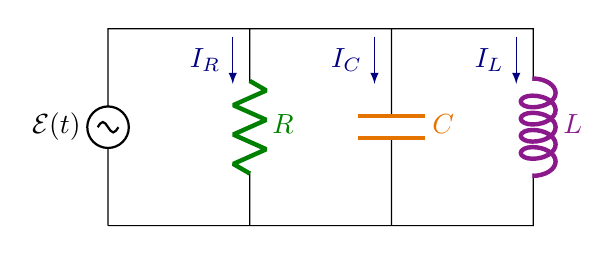
\begin{tikzpicture}
  \def\ang{155}
  \def\a{0.9}
  \def\b{0.8}
  \def\h{2.5}
  \def\w{1.8}
  \draw (0,0) to[AC] (0,\h) --
        (3*\w,\h) to[thick L] ++(0,-\h) -- (0,0)
        (1*\w,\h) to[thick R] ++(0,-\h)
        (2*\w,\h) to[thick C] ++(0,-\h);
  \draw[->,Icol] (0.88*\w,0.96*\h) --++ (0,-0.24*\h) node[midway,left=1] {$I_R$};
  \draw[->,Icol] (1.88*\w,0.96*\h) --++ (0,-0.24*\h) node[midway,left=1] {$I_C$};
  \draw[->,Icol] (2.88*\w,0.96*\h) --++ (0,-0.24*\h) node[midway,left=1] {$I_L$};
  %\node[minuscol,scale=0.8,align=right] at (2.95,0.55) {$-Q(t)$};
  %\node[pluscol,scale=0.8,align=right] at (2.95,1.45) {$+Q(t)$};
\end{tikzpicture}


% AC, RCL series
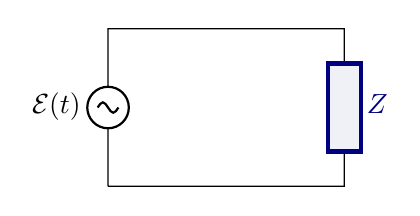
\begin{tikzpicture}
  \def\ang{120}
  \def\a{1.0}
  \def\b{0.8}
  \draw (0,0) to[AC] (0,2) --++(3,0)
              to[thick Z] ++(0,-2) -- (0,0);
\end{tikzpicture}


\end{document}
